\newpage
\changefontsizes{16pt}
\centerline{\textbf{\hyperlink{page.6}{CHƯƠNG 3: THỰC NGHIỆM}}}

%
\bigskip
\changefontsizes{14pt}

\leftskip0cm
\setlength{\parindent}{0.0cm}
\textbf{3.1 Dữ liệu.}

\smallskip
\changefontsizes{13pt}
\setlength{\parindent}{1cm}
\leftskip0cm

%fill here
Các testcase được tìm kiếm trên mạng hoặc do chính người lập trình nghĩ ra để test nhiều trường hợp khác nhau. Khi báo cáo có thể sẽ có thêm nhiều testcase khác do người hướng dẫn cung cấp.

\bigskip
\changefontsizes{14pt}

\setlength{\parindent}{0.0cm}
\textbf{3.2 Công nghệ.}


\smallskip
\changefontsizes{14pt}

\setlength{\parindent}{0.5cm}
\textbf{3.2.1 Ngôn ngữ lập trình.}

\smallskip
\changefontsizes{13pt}
\setlength{\parindent}{1cm}

\leftskip0.5cm
Ngôn ngữ lập trình được sử dụng trong bài báo cáo này là Python. Ngoài việc Python là ngôn ngữ bắt buộc khi học môn học này thì nó đang dần trở nên phổ biến hơn ngày nay. Sự phát triển của nhiều ngành như trí tuệ nhân tạo, học máy một cách nhanh chóng, các thuật toán ngày càng trở nên tinh vi hơn thì việc sử dụng Python sẽ giúp chúng ta tiếp cận mọi thứ một cách dễ dàng, hiệu quả hơn. Ngoài ra, Python còn rất dễ sử dụng, dễ cài đặt, vì thế nên nó càng trở nên dễ tiếp cận với mọi người.
%fill here


\leftskip0cm
\bigskip
\changefontsizes{14pt}


\setlength{\parindent}{0.5cm}
\textbf{3.2.2 Thư viện.}

\smallskip
\changefontsizes{13pt}
\setlength{\parindent}{1cm}
\leftskip0.5cm

%fill here
Bài báo cáo chỉ gồm 3 bài tập theo yêu cầu và đây lại là môn học phân tích và thiết kế giải thuật nên bài báo cáo không sử dụng thư viện nào hổ trợ. Đây lại là những bài toán cơ bản, điển hình cho chủ đề của đồ án nên việc sử dụng thư viện có thể không cần thiết, sinh viên có thể tự hoàn thiện code của mình mà không cần thư viện.


\leftskip0cm
\bigskip
\changefontsizes{14pt}

\setlength{\parindent}{0.0cm}
\textbf{3.3 Thực nghiệm.}

\smallskip
\changefontsizes{14pt}

\setlength{\parindent}{0.5cm}
\textbf{3.3.1 Bài toán dãy con tăng dài nhất.}

\smallskip
\leftskip0.5cm
\changefontsizes{13pt}
\textbf{Ý tưởng}


\leftskip1.5cm
\setlength{\parindent}{0cm}
- Tạo một mảng lưu giá trị của từng phần tử trong dãy số, có giá trị đầu là 0.

- Duyệt dãy số từ cuối ngược lên đầu. Tại mỗi phần tử, giá trị mới của nó bằng giá trị lớn nhất trong số các phần tử lớn hơn nó cộng thêm 1.

- Từ mảng các giá trị chọn ra dãy con tăng dài nhất của dãy số.


\begin{figure}[h!]
	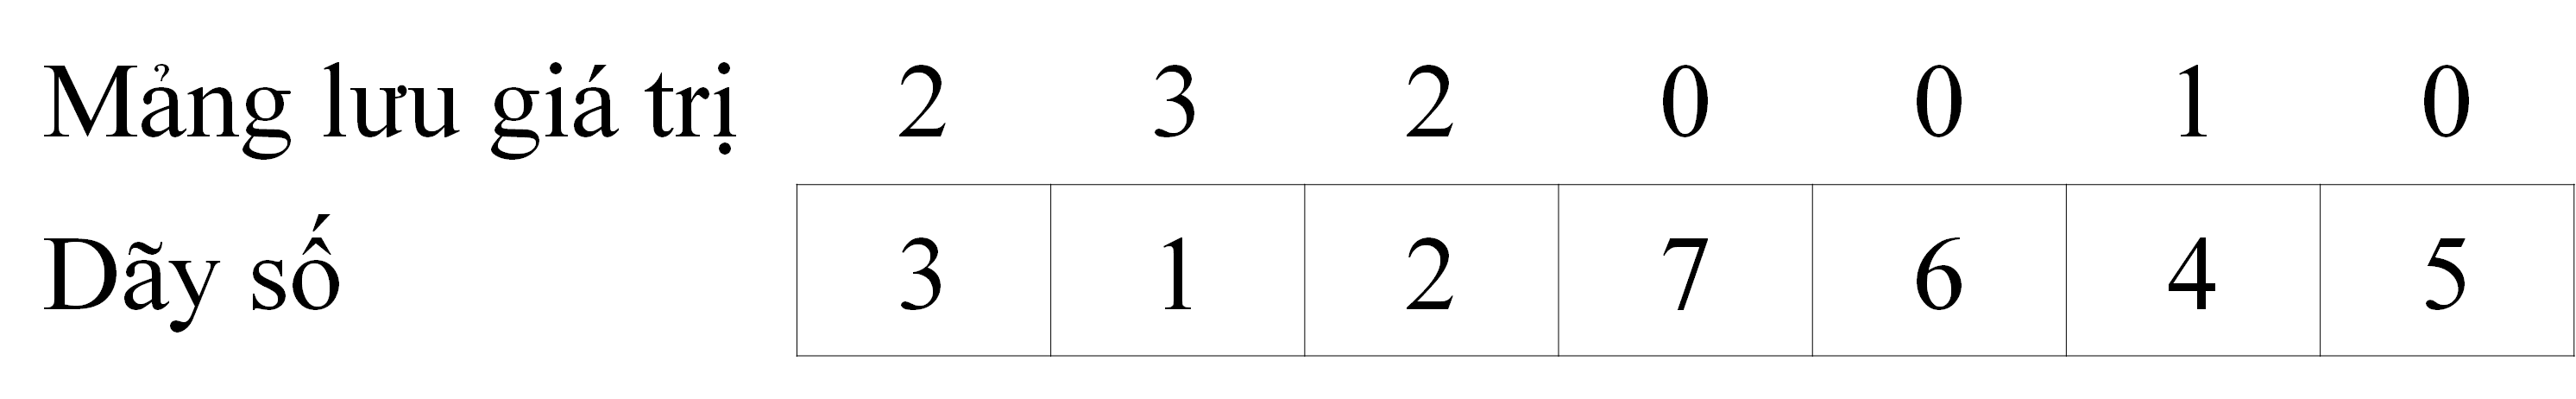
\includegraphics[scale=0.2]{./image/LCS.png}
	\caption{Mảng giá trị của dãy số.}
\end{figure}


\leftskip1cm

\setlength{\parindent}{0cm}
\textbf{Mã giả}

\smallskip
\leftskip1.5cm


\begin{minipage}{.9\linewidth}
	\begin{algorithm}[H]
		\SetKwInOut{Input}{Đầu vào}
		\SetKwInOut{Output}{Đầu ra}
		\SetKwProg{Algorithm}{function LIS}{}{}
		\Algorithm{$(array)$}
		{ 
			\Input{Mảng các số nguyên}
			\Output{Chuỗi con tăng dài nhất}
			
			$val$ is an array of $n$ zeros;
			
			\For{$i \leftarrow n - 1$ \KwTo $0$}{
				\For{$j \leftarrow i$ \KwTo $n - 1$}{
					\If{$array_j > array_i$ \textbf{and} $val_j \geq val_i$  }
					{$val_i \leftarrow val_j + 1$;}
				}
			}
			
			$lis$ is an interger array;
			
			$m \leftarrow max(val)$;
			
			\For{$i \leftarrow i$ \KwTo $n - 1$}{
				\If{$val_i = m$  }	{
					$lis$.Insert($array$($i$));
					
					$m \leftarrow m - 1$
				}
				
			}
			
			\Return{$lis$}
		}
		\caption{Chuỗi con tăng dài nhất}
		\label{alg:algorithm1}
	\end{algorithm}
\end{minipage}




\leftskip0cm


\bigskip
\changefontsizes{14pt}
\setlength{\parindent}{0.5cm}
\textbf{3.3.2 Bài toán dãy con chung dài nhất LCS.}


\smallskip
\leftskip0.5cm
\changefontsizes{13pt}
\textbf{Ý tưởng}


\leftskip1.5cm
\setlength{\parindent}{0cm}
- Hai chuỗi đầu vào sẽ được tách nhỏ ra để tìm kiếm dãy con chung dài nhất sau đó tổng hợp lại và chọn chuỗi dài nhất mà hàm tìm được.

- Bài toán sẽ được giải theo đệ quy với điều kiện dừng là khi một trong hai (hoặc cả hai) chuỗi không còn ký tự để so sánh.


\vspace{-0.5cm}
\begin{figure}[h!]
	\includegraphics[scale=0.3675]{./image/LCSo.png}
	\caption{Minh họa hàm đệ quy LCS.}
\end{figure}


\leftskip1cm


\setlength{\parindent}{0cm}
\textbf{Mã giả}


\smallskip
\leftskip1.5cm


\begin{minipage}{.9\linewidth}
	\begin{algorithm}[H]
		\SetKwInOut{Input}{Đầu vào}
		\SetKwInOut{Output}{Đầu ra}
		\SetKwProg{Algorithm}{function LCS}{}{}
		\Algorithm{$(str1, str2, lcs)$}
		{ 
			\Input{2 chuỗi cần tìm dãy con chung và 1 biến lưu giá trị}
			\Output{Chuỗi con chung dài nhất}
			
			\If{$str1 = 0 $ \textbf{or} $ str2 = 0$}
			{\textbf{return} $lcs$;}
			
			\If{$str1[0] = str2[0]$}
			{
				$str1.Remove(str1[0])$;\\
				$str2.Remove(str2[0])$;\\
				$lcs \leftarrow lcs + str1[0]$;\\
				\textbf{return} LCS($str1, str2, lcs$);}
			\Else{
				$newstr1 = str1$;\\
				$newstr1.remove(str1[0])$;\\
				$child1 = $LCS($newstr1, str2, lcs$);\\
				$newstr2 = str2$;\\
				$newstr2.remove(str2[0])$;\\
				$child2 = $LCS($str1, newstr2, lcs$);\\
				\textbf{return} max($child1, child2,$ key=length);
			}
			
		}
		\caption{Chuỗi con chung dài nhất}
		\label{alg:algorithm1}
	\end{algorithm}
\end{minipage}




\leftskip0cm
\setlength{\parindent}{0.5cm}

\bigskip
\changefontsizes{14pt}
\textbf{3.3.3 Bài toán cây nhị phân vô hạn.}



\smallskip
\leftskip0.5cm
\changefontsizes{13pt}
\textbf{Ý tưởng}

\leftskip1.5cm

\setlength{\parindent}{0cm}


- Chuỗi lưu các node trên cây trong cuộc dạo chơi sẽ được cắt thành các cuộc dạo chơi ngắn hơn sau đó tổng hợp lại để tính giá trị cuối cùng.

- Dùng một biến lưu trữ giá trị hiện thời của node, với giá trị đầu là 1.


\vspace{-0.5cm}
\begin{figure}[h!]
	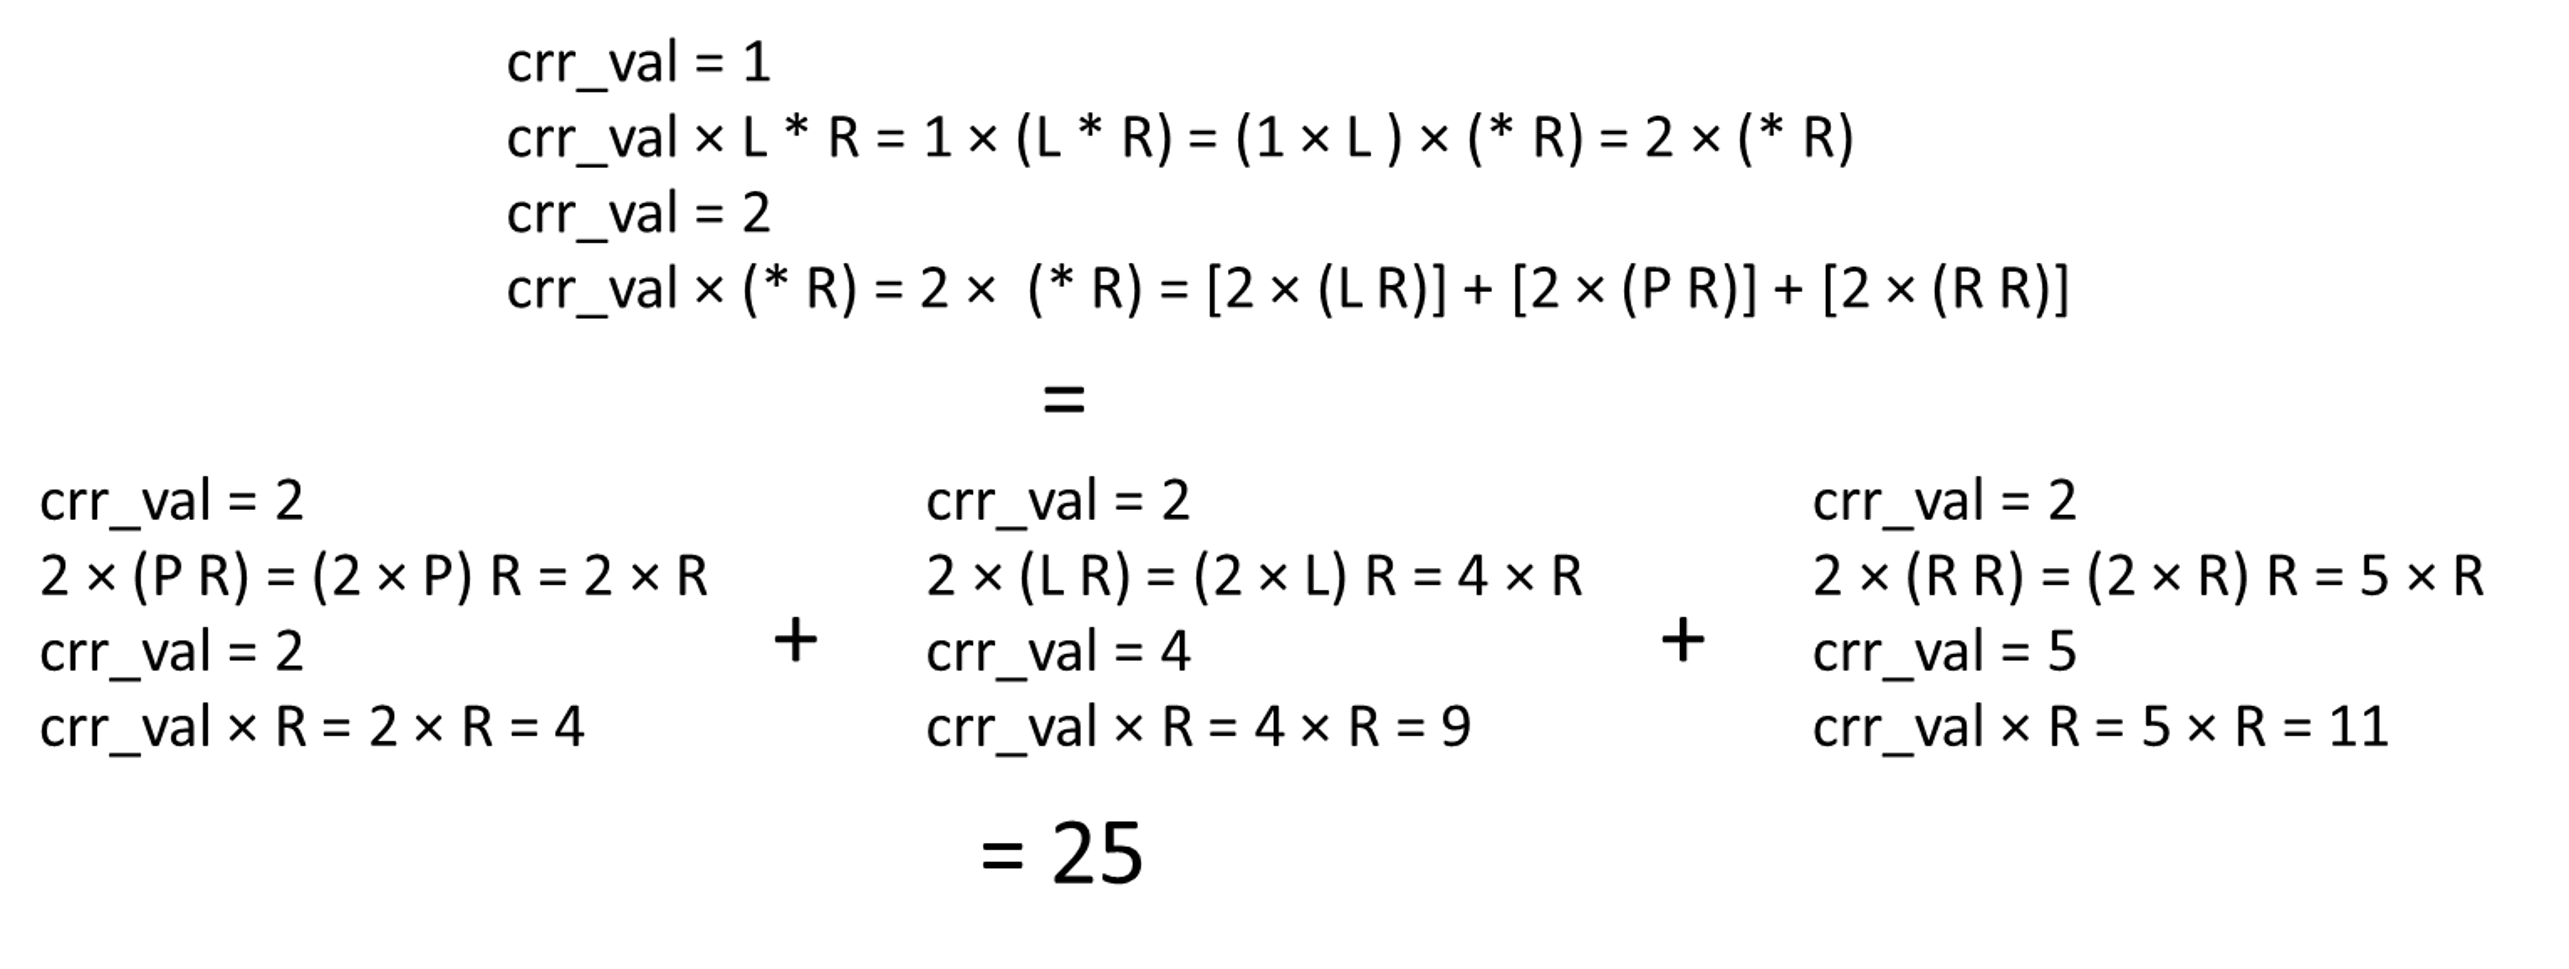
\includegraphics[scale=0.3]{./image/tree.png}
	\caption{Minh họa cách tính giá trị của chuyến đi trên cây.}
\end{figure}

\leftskip0cm


\leftskip1cm
\setlength{\parindent}{0cm}
\textbf{Mã giả}


\leftskip1.5cm



\begin{minipage}{.9\linewidth}
	\begin{algorithm}[H]
		\SetKwInOut{Input}{Đầu vào}
		\SetKwInOut{Output}{Đầu ra}
		\SetKwProg{Algorithm}{function inf\_tree}{}{}
		\Algorithm{$(str, crr\_val)$}
		{ 
			\Input{1 chuỗi lưu các node và 1 biến lưu giá trị}
			\Output{Giá trị cuối cùng của chuyến dạo chơi}
			
			\If{$str$\textbf{.isEmpty()}}
			{\textbf{return} $crr\_val$;}
			
			$crr\_pos \leftarrow str[0]$;\\
			$str.Remove(str[0])$
			
			\If{$crr\_pos = $ 'P'}
			{
				\textbf{return} inf\_tree($str, crr\_val$);}
			\ElseIf{$crr\_pos = $ 'L'}{
				\textbf{return} inf\_tree($str, crr\_val \times 2$);
			}
			\ElseIf{$crr\_pos = $ 'R'}{
				\textbf{return} inf\_tree($str, crr\_val \times 2 + 1$);
			}
			\ElseIf{$crr\_pos = $ '*'}{
				$P \leftarrow $inf\_tree($str, crr\_val$);\\
				$L \leftarrow $inf\_tree($str, crr\_val \times 2$);\\
				$R \leftarrow $inf\_tree($str, crr\_val \times 2 + 1$);\\
				\textbf{return} $P + L + R$;
			}
			
		}
		\caption{Cây nhị phân vô hạn}
		\label{alg:algorithm1}
	\end{algorithm}
\end{minipage}




\leftskip0cm

\bigskip
\changefontsizes{14pt}

\setlength{\parindent}{0.0cm}
\textbf{3.4 Đánh giá kết quả.}
\setlength{\parindent}{1.0cm}

\smallskip
\changefontsizes{13pt}

%fill here
Từ những thực nghiệm đã được nêu như trên có thể rút ra đánh giá cho bài báo cáo là cơ bản hoàn thành các yêu cầu của đồ án. Bài báo cáo đã test qua nhiều testcase khác nhau và chính xác ở mọi trường hợp được test. Phương pháp quy hoạch động cũng được chỉ ra ở phần code trên. Vì vậy, đây có thể coi là kết quả tương đối tốt cho bài báo cáo này, hoàn thành không chỉ yêu cầu về mặt kết quả mà còn về mặt thuật toán.
%


